

% ----- APÊNDICE 1 - CATALOGAÇÃO DA USINA SOLAR -----
\clearpage % garante que começa em página nova
\phantomsection % marca link para o sumário correto
\label{ap:catalogacao-u}
\addcontentsline{toc}{chapter}{APÊNDICE 1 - CATALOGAÇÃO DA USINA SOLAR} % adiciona ao sumário



\vspace*{\fill} % centraliza verticalmente
\begin{center}
    {\LARGE \textbf{APÊNDICE 1}}\\[1\baselineskip]
    {\LARGE \textbf{CATALOGAÇÃO DA USINA SOLAR}}
\end{center}
\vspace*{\fill}




\clearpage % próxima página começa depois do anexo

%\section*{Conteúdo do Anexo}
%\addcontentsline{toc}{section}{Conteúdo do Anexo} % se quiser adicionar subtítulo ao sumário
%Aqui vai o conteúdo do anexo, imagens, figuras, tabelas etc.

%\captionsetup[figure]{name=Anexo} % muda o nome apenas para a próxima figura

\begin{figure}[h!]
\centering
\hspace*{-2.7cm}
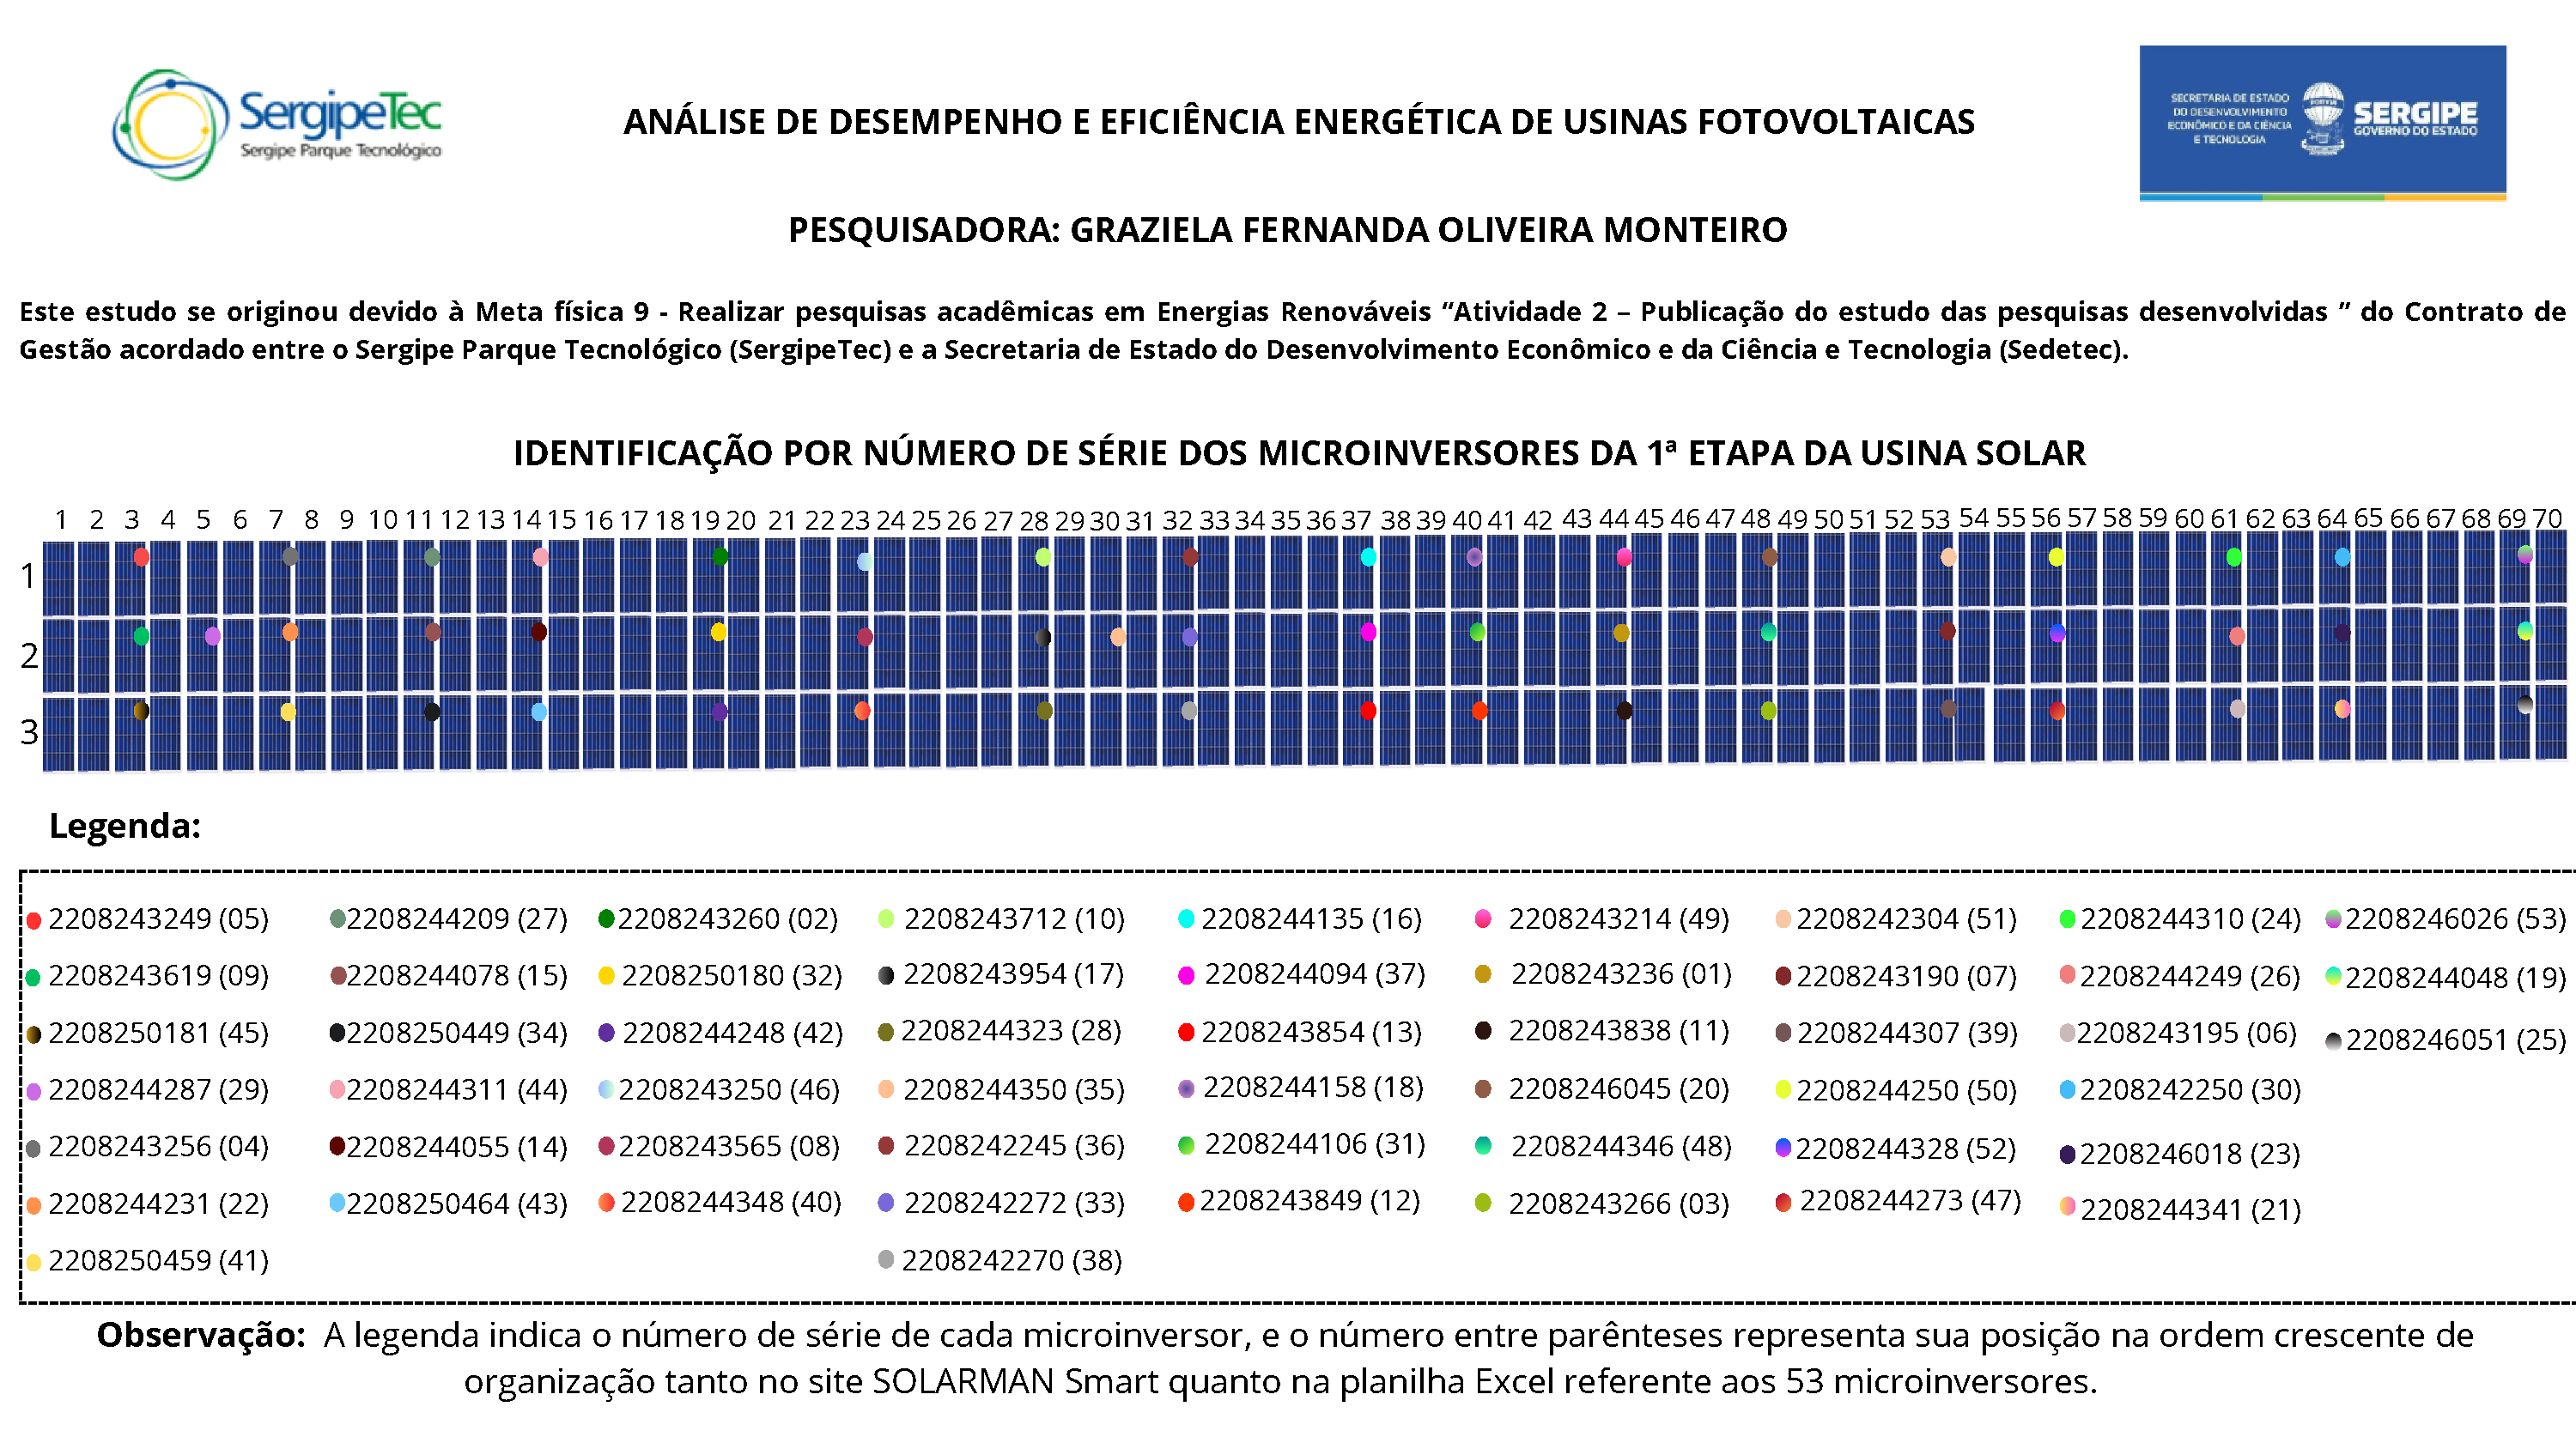
\includegraphics[page=1, width=1.25\textwidth]{Anexos/CATALOGAÇÃO DA USINA SOLAR DO SERGIPETEC - 1ª ETAPA - GERAL.pdf}
\caption*{}
\label{fig:pdfpag1}
\end{figure}




% ---- restaurar o nome padrão ----
\captionsetup[figure]{name=Figura}

\begin{figure}[h!]
    \centering
    \vspace{-1cm}
    \hspace*{-2.7cm}
    \includegraphics[page=2, width=1.25\textwidth]{Anexos/CATALOGAÇÃO DA USINA SOLAR DO SERGIPETEC - 1ª ETAPA - GERAL.pdf}
    \caption*{}
    \label{fig:pdfpag2}
\end{figure}

\begin{figure}[h!]
    \centering
    \hspace*{-2.7cm}
    \includegraphics[page=3, width=1.25\textwidth]{Anexos/CATALOGAÇÃO DA USINA SOLAR DO SERGIPETEC - 1ª ETAPA - GERAL.pdf}
    \caption*{}
    \label{fig:pdfpag3}
\end{figure}

\begin{figure}[h!]
    \centering
    \hspace*{-2.7cm}
    \includegraphics[page=4, width=1.25\textwidth]{Anexos/CATALOGAÇÃO DA USINA SOLAR DO SERGIPETEC - 1ª ETAPA - GERAL.pdf}
    \caption*{}
    \label{fig:pdfpag4}
\end{figure}

\clearpage
\vspace*{-\topskip}
\begin{center}
    \hspace*{-2.7cm}
    \includegraphics[page=5, width=1.25\textwidth]{Anexos/CATALOGAÇÃO DA USINA SOLAR DO SERGIPETEC - 1ª ETAPA - GERAL.pdf}
\end{center}






























% ----- ANEXO 1 - Manual e datasheet do carport solar -----
\clearpage % garante que começa em página nova
\phantomsection % marca link para o sumário correto
\label{ap:datasheet-carport}
\addcontentsline{toc}{chapter}{ANEXO 1 - MANUAL E DATASHEET DO CARPORT SOLAR} % adiciona ao sumário



\vspace*{\fill} % centraliza verticalmente
\begin{center}
    {\LARGE \textbf{ANEXO 1}}\\[1\baselineskip]
    {\LARGE \textbf{MANUAL E DATASHEET DO CARPORT SOLAR}}

    
\end{center}
\vspace*{\fill}




\newpage % próxima página começa depois do anexo

%section*{Conteúdo do Anexo}
%addcontentsline{toc}{section}{Conteúdo do Anexo} % se quiser adicionar subtítulo ao sumário
%Aqui vai o conteúdo do anexo, imagens, figuras, tabelas etc.

\captionsetup[figure]{name=Anexo} % muda o nome apenas para a próxima figura

    \vspace*{0cm}
    \centering
    \hspace*{-1.5cm}
    \includegraphics[page=1, width=1.1\textwidth]{Anexos/Manual - Garagem - Carport Solar RS-401 .pdf}
    \label{fig:pdfpag1}


    
    \vspace*{-2cm}
    \centering
    \hspace*{-1.5cm}
    \includegraphics[page=2, width=1.1\textwidth]{Anexos/Manual - Garagem - Carport Solar RS-401 .pdf}
    \label{fig:pdfpag1}


    \vspace*{-2cm}
    \centering
    \hspace*{-1.5cm}
    \includegraphics[page=3, width=1.1\textwidth]{Anexos/Manual - Garagem - Carport Solar RS-401 .pdf}
    \label{fig:pdfpag1}



    \vspace*{-2cm}
    \centering
    \hspace*{-1.5cm}
    \includegraphics[page=4, width=1.1\textwidth]{Anexos/Manual - Garagem - Carport Solar RS-401 .pdf}
    \label{fig:pdfpag1}




\begin{figure}[h!]
    \centering
    \hspace*{-2.7cm}
    \includegraphics[page=1, width=1.25\textwidth]{Anexos/RS-401 (CLIENTE).pdf}
    \caption*{}
    \label{fig:pdfpag1}
\end{figure}


\begin{figure}[h!]
    \centering
    \hspace*{-2.7cm}
    \includegraphics[page=2, width=1.25\textwidth]{Anexos/RS-401 (CLIENTE).pdf}
    \caption*{}
    \label{fig:pdfpag1}
\end{figure}



\begin{figure}[h!]
    \centering
    \hspace*{-2.7cm}
    \includegraphics[page=3, width=1.25\textwidth]{Anexos/RS-401 (CLIENTE).pdf}
    \caption*{}
    \label{fig:pdfpag1}
\end{figure}


\begin{figure}[h!]
    \centering
    \hspace*{-2.7cm}
    \includegraphics[page=4, width=1.25\textwidth]{Anexos/RS-401 (CLIENTE).pdf}
    \caption*{}
    \label{fig:pdfpag1}
\end{figure}














% ----- ANEXO 2 - DATASHEET DOS MÓDULOS FOTOVOLTAICOS -----
\clearpage % garante que começa em página nova
\phantomsection % marca link para o sumário correto
\label{ap:datasheet-modulos}
\addcontentsline{toc}{chapter}{ANEXO 2 - DATASHEET DOS MÓDULOS FOTOVOLTAICOS} % adiciona ao sumário



\vspace*{\fill} % centraliza verticalmente
\begin{center}
    {\LARGE \textbf{ANEXO 2}}\\[1\baselineskip]
    {\LARGE \textbf{DATASHEET DO MÓDULO FOTOVOLTAICO}}
\end{center}
\vspace*{\fill}




\clearpage % próxima página começa depois do anexo

%\section*{Conteúdo do Anexo}
%\addcontentsline{toc}{section}{Conteúdo do Anexo} % se quiser adicionar subtítulo ao sumário
%Aqui vai o conteúdo do anexo, imagens, figuras, tabelas etc.

%\captionsetup[figure]{name=Anexo} % muda o nome apenas para a próxima figura

\clearpage
\vspace*{-2cm}
\centering
\hspace*{-2.0cm}
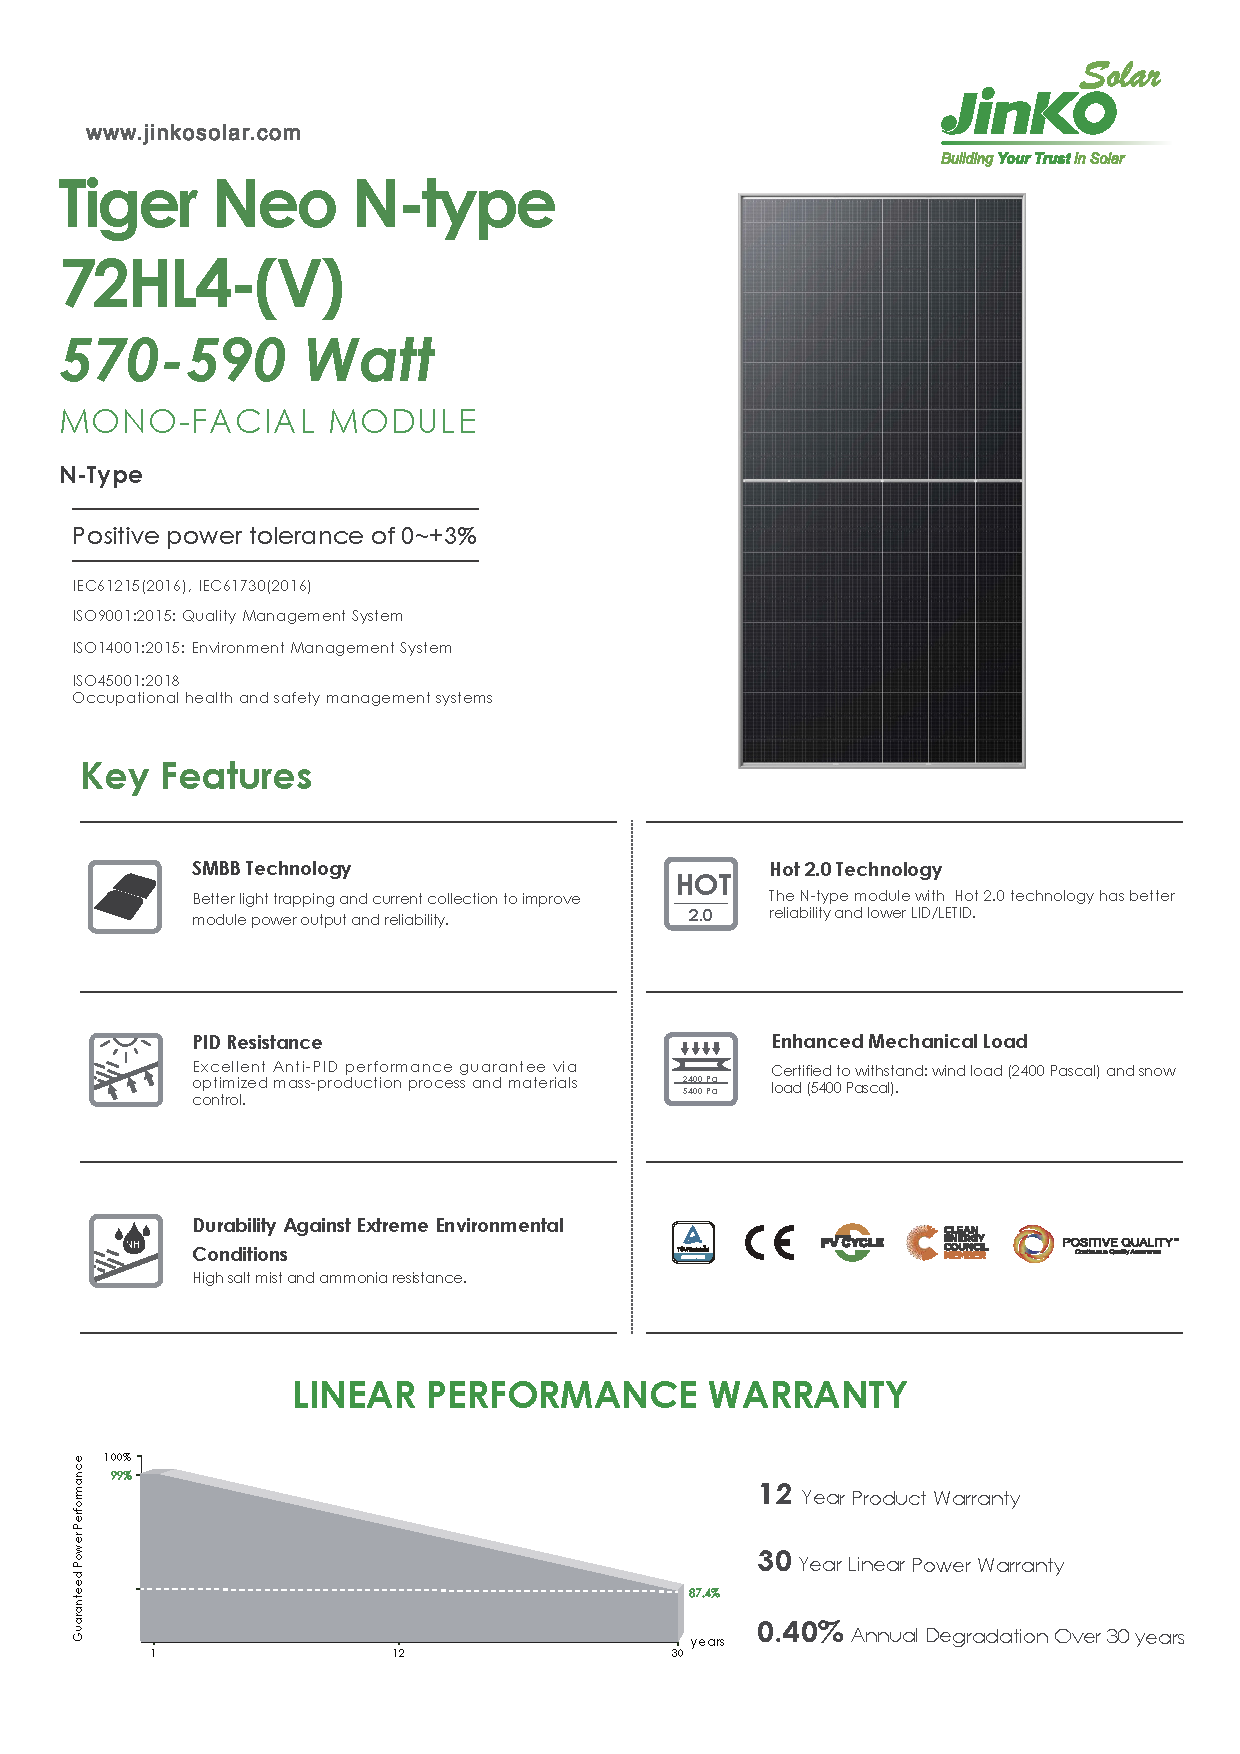
\includegraphics[page=1, width=1.15\textwidth]{Anexos/DATASHEET- JINKO 580W.pdf}
\label{fig:pdfpag1}




\vspace*{-2cm}
\centering
\hspace*{-2.0cm}
\includegraphics[page=2, width=1.15\textwidth]{Anexos/DATASHEET- JINKO 580W.pdf}
\label{fig:pdfpag1}

















% ----- ANEXO 3 - DATASHEET DOS MICROINVERSORES -----
%\newpage % garante que começa em página nova
\phantomsection % marca link para o sumário correto
\label{ap:datasheet-microinversores}
\addcontentsline{toc}{chapter}{ANEXO 3 - DATASHEET DOS MICROINVERSORES} % adiciona ao sumário



\vspace*{\fill} % centraliza verticalmente
\begin{center}
    {\LARGE \textbf{ANEXO 3}}\\[1\baselineskip]
    {\LARGE \textbf{DATASHEET DO MICROINVERSOR}}
\end{center}
\vspace*{\fill}




\clearpage % próxima página começa depois do anexo

%\section*{Conteúdo do Anexo}
%\addcontentsline{toc}{section}{Conteúdo do Anexo} % se quiser adicionar subtítulo ao sumário
%Aqui vai o conteúdo do anexo, imagens, figuras, tabelas etc.

%\captionsetup[figure]{name=Anexo} % muda o nome apenas para a próxima figura

\begin{figure}[h!]
    \centering
    \hspace*{-2.7cm}
    \includegraphics[page=1, width=1.25\textwidth]{Anexos/DATASHEET - MICROINVERSOR DEYE 2kW.pdf}
    \caption*{}
    \label{fig:pdfpag1}
\end{figure}















